\documentclass[TD, noCustomPackages]{UPSTI_Document}
\usepackage{IUT_Annecy}
\usepackage{logos_iut}

% --- Git info (nécessite git et les hooks gitinfo2 activés) ---
\usepackage{gitinfo2} % génère gitHeadInfo.gin via hooks post-commit/checkout/merge
% Voir doc gitinfo2 pour activer les hooks une fois:
%   git config --local gitinfo2.enabled true
%   git info # ou copier les hooks fournis par le package
\newcommand{\sequence}{P}
\newcommand{\UPSTIsousTitreEnTete}{Hackathon 1}

\graphicspath{{images/}}



\discipline{Informatique}
\newcommand{\UPSTIidClasse}{1}
\newcommand{\UPSTItitreEnTete}{Informatique}


%\newcommand{\UPSTIsource}{Certaines images proviennent du site freepics.com}

\usepackage{listings}
\usepackage{xcolor}
\usepackage{amssymb} % pour \Box et \CheckedBox
\usepackage{makecell} % permet \makecell{...} avec des \\ dans une cellule
\renewcommand\arraystretch{1.2}

\lstdefinelanguage{bash}{
  alsoletter={-},           % autoriser "-" dans les mots-clés
  morekeywords={
    ls, cd, mv, cp, rm, mkdir, rmdir, echo, cat, less, head, tail,
    grep, find, chmod, chown, ps, kill, top, man, which, alias, export,
    ssh, scp, rsync, tar, gzip, gunzip, ping, curl, wget, zip, unzip, code
  },
  sensitive=true,           % sensible à la casse
  morecomment=[l]{\#},      % commentaires avec #
  morestring=[b]",          % chaînes "..."
  morestring=[b]'           % chaînes '...'
}

\definecolor{colString}{rgb}{0.6,0.1,0.1}
\definecolor{lightblack}{rgb}{0.3,.3,.3}

\newcommand{\prompt}[1]{\textcolor{gray}{#1}}

% \lstdefinestyle{console}{
%   language=bash,
%   basicstyle=\ttfamily,
%   columns=fullflexible,
%   keepspaces=true,
%   escapeinside=||, % <- permet d'injecter du LaTeX entre |...|
% }

\lstdefinestyle{console}{
    basicstyle      = \footnotesize\ttfamily,% ecriture standard
    extendedchars   = true,% permet d'avoir des accents dans le code
    tabsize         = 2,%
    showspaces      = false,%
    showstringspaces = false,%
    numbers=none,%
    breaklines=true,%
    breakautoindent=true,%
    escapeinside=|| % <- permet d'injecter du LaTeX entre |...|
}




\documentVersion{E}
\newcommand{\UPSTInumeroVersion}{\gitAuthorDate\if \gitDirty*dirty \fi}
\newcommand{\UPSTInumero}{\sequence.9}
\usepackage{eso-pic}
\begin{document}
% QR code (marqueur pédagogique) : superposition additive en bas à droite de chaque page via eso-pic.
% Source unique du texte : ../_commun/images/marqueur_qr.txt -- partagé par
% tous les projets (modifier uniquement ce .txt, jamais le .png, puis
% régénérer le QR depuis 99_Projets/_commun/ avec :
%   qrencode -8 -o images/marqueur_qr.png -s 10 -l H -r images/marqueur_qr.txt
\AddToShipoutPictureFG{%
    \AtPageLowerLeft{\put(\LenToUnit{\paperwidth-1.1cm},\LenToUnit{0.35cm}){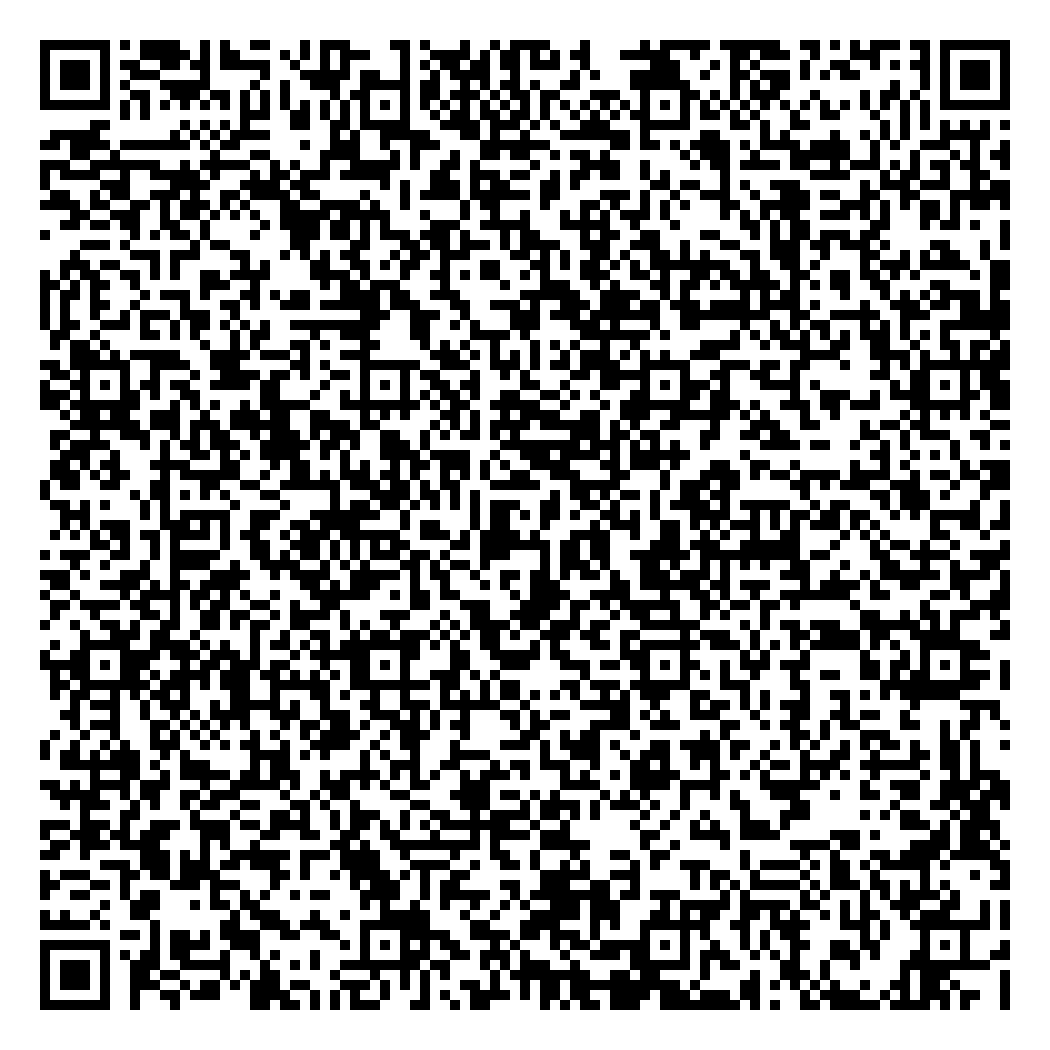
\includegraphics[height=0.7cm]{../_commun/images/marqueur_qr.png}}}%
}
\AddToShipoutPictureFG{%
    \AtPageUpperLeft{\put(\LenToUnit{1.5cm},\LenToUnit{-1cm}){%
        \parbox{15cm}{\tiny\color{white}\input{../_commun/images/marqueur_qr.txt}}%
    }}%
}

\tableofcontents
\pagebreak
\section{Projet 9 — Le bandit manchot}
\setcounter{UPSTInumeroCahier des charges}{0}

\subsection*{Objectif du jeu}
Simuler un bandit manchot (machines à sous) à 3 rouleaux et gérer le capital du joueur selon les combinaisons obtenues.


\subsection*{Règles du jeu}
\begin{itemize}
  \item 3 \textbf{rouleaux} de 11 figures (tableau 2D). Codes : \texttt{7, B, L, C} (sept, barre, citron, cerise).
  \item Le joueur commence avec \textbf{100 points} et mise 1 ou 3 points.
  \item Appui sur \texttt{J} : tirage aléatoire d’une figure par rouleau; affichage en ligne des trois codes.
  \item Le joueur gagne si une des combinaisons ci-dessous apparaît (\textbf{peu importe l'ordre}), sinon il perd sa mise ; le capital est mis à jour ; le joueur peut continuer (\texttt{O/N}).
\end{itemize}

\subsection*{Les rouleaux et les combinaisons}
\begin{center}
  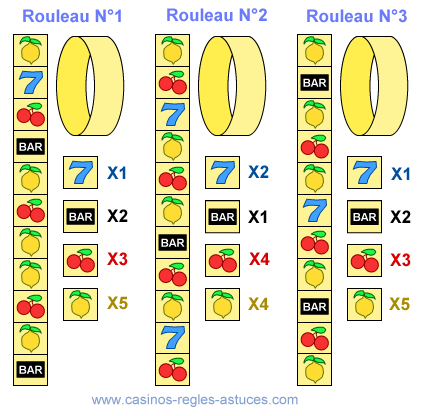
\includegraphics[width=0.7\textwidth]{sources/images/bandit_manchot_rouleaux.png}
\end{center}
Dans le programme : 7 est mémorisé par \texttt{'7'}, BAR par \texttt{'B'}, cerise par \texttt{'C'}, citron par \texttt{'L'}.

\textit{Conseils :} ranger les 3 figures tirées dans un tableau ; en mode test, vous pouvez modifier les rouleaux pour favoriser une combinaison.

\subsection*{Cahier des charges}
\begin{UPSTICahierDesCharges}{1}
\begin{itemize}
  \item Initialiser les \textbf{3 rouleaux} (tableau 3×11) et afficher leur contenu pour vérification.
  \item Tirer et afficher \textbf{une figure par rouleau} (codes).
  \item Mettre à jour le capital selon résultat simple (ex.\,égalité des 3).
\end{itemize}
\end{UPSTICahierDesCharges}

\begin{UPSTICahierDesCharges}{2}
\begin{itemize}
  \item Implémenter les \textbf{mises} (1 ou 3), détailler les combinaisons gagnantes/perdantes.
  \item Si aucune combinaison n'apparaît, le joueur peut \textbf{rejouer} un ou plusieurs rouleaux (ex.\,saisie \texttt{23} pour rejouer les rouleaux 2 et 3, puis \texttt{J}) ; il perd alors 1 point (ou 3 selon la mise de départ). Et ainsi de suite jusqu'à obtenir une combinaison ou ne plus avoir de points.
  \item Récapitulatif clair de fin.
\end{itemize}
\end{UPSTICahierDesCharges}

\begin{UPSTICahierDesCharges}{3}
\begin{itemize}
  \item Présentation et rejouabilité; options de test (rouleaux biaisés).
  \item Structuration en fonctions (tirage, calcul gain, affichage).
  \item Robustesse des saisies.
\end{itemize}
\end{UPSTICahierDesCharges}




\end{document}
